\section{Instrukcja użycia języka}

Głównym elementem języka jest \textbf{obiekt}. Obiekty mogą posiadać nazwę. Właściwości obiektu definiuje się za pomocą \textbf{par klucz-wartość}. Ważną właściwością obiektu jest nazwa obiektu bazowego, tj. obiektu który jest prototypem dla danego obiektu.

\begin{lstlisting}
class Klasa
	name: "Moja Klasa"
	stereotype: "Fajna"
\end{lstlisting}

Przykładem jest obiekt o nazwie ,,Klasa''. Jego prototypem jest obiekt o nazwie ,,class'', zdefiniowany w \textbf{bibliotece standardowej}. ,,Klasa'' posiada dwie pary klucz-wartość: ,,name'' oraz ,,stereotype''.

\subsection{Prototypy}

W powyższym przykładzie pokazaliśmy obiekt bazujący na obiekcie ,,class''. ,,class'' jest tzw. prototypem, zdefiniowanym następująco:

\begin{lstlisting}
prototype base class
    allow name STRING
    allow stereotype STRING
\end{lstlisting}

Słowo kluczowe \textbf{prototype} sprawi, że obiekt będzie ignorowany przez moduł rysujący diagram. Stanie się ,,niewidocznym obiektem'' używanym jako obiekt bazowy. \textbf{base} mówi, że obiekt nie bazuje na żadnym innym obiekcie. Deklaracje \textbf{allow} definiują ograniczenia nałożone na obiekty bazujące na tym prototypie. Sprawiają, ze bazując na ,,class'' będzie można ustawiać tylko klucze ,,name'' oraz ,,stereotype'' które mogą być typu \textbf{STRING} czyli ciąg znaków.

\subsubsection{Ograniczenia prototypów}

\emph{Uwaga - dalsza wiedza o prototypach nie jest potrzebna do wygodnego użytkowania programu.}

Oprócz \textbf{allow} można używać również \textbf{require}. \textbf{Require} sprawi, że użytkownik będzie zmuszony ustawić podany klucz, inaczej kompilacja diagramu nie powiedzie się.

Przykład \textbf{require}:
\begin{lstlisting}
prototype base relation
    require source-object OBJECT
    require target-object OBJECT
\end{lstlisting}

Poznaliśmy właśnie kolejny rodzaj wartości jaką można ustawić klucz - \textbf{OBJECT}. Wartość oczekiwana w tym wypadku to nazwa zdefiniowanego wcześniej obiektu, np. (ale niekoniecznie) prototypu.

Dozwolone ograniczenia na wartości to:
\begin{itemize}
	\item STRING - ciąg znaków
	\item OBJECT - nazwa zdefiniowanego obiektu
	\item MULTIPLICITY - UMLowa krotność, czyli liczba lub zakres, dozwolony znak *
	\item Lista wartości - lista dozwolonych identyfikatorów podawana w formacie: [a, b, c].
\end{itemize}

\subsubsection{,,Metody'' oraz ,,Atrybuty'' dla klas UML}

Język \omlet umożliwia definiowanie klas oraz atrybutów notacji UML. Wg przykładu:
\begin{lstlisting}
	+metoda(argument) : typ
    -atrybut : typ = "wartosc"
    _+statyczna_metoda()
\end{lstlisting}

\textbf{+} lub \textbf{-} przed nazwą metody/atrybutu oznacza widoczność (\emph{public} lub \emph{private}). \textbf{\_} przed widocznością pozwala zaznacza, że metoda jest statyczna. Po \textbf{:} można zdefiniować typ oraz, dla atrybutów, domyślną wartość.

\subsection{Dziedziczenie}

Tworząc obiekt bazujący na innym obiekcie (prototypie), obiekt przejmuje wszystkie ustawione klucze. Spójrzmy na przykład prototypu z ustawionymi kluczami:

\begin{lstlisting}
prototype relation generalization
    arrow: "generalization"
    direction: target
\end{lstlisting}

Teraz definiując obiekt bazujący na prototypie ,,generalization'', automatycznie przejmujemy wartości dla kluczy ,,arrow'' oraz ,,direction''. Znacznie ułatwia to tworzenie samych diagramów.

\subsection{Typy wbudowane}

Typem wbudowanym nazywamy obiekty które są interpretowane przez \omlet \footnote{A mianowicie moduł \textbf{DrawableFactory}} i potrafią być reprezentowane przez fizyczny \footnote{instancja pochodnych klasy Drawable} obiekt na diagramie. Dostępne typy wbudowane to:

\begin{itemize}
	\item actor
	\item class
	\item usecase
	\item note
	\item relation
\end{itemize}

Każdy z typów wbudowanych rysuje elementy diagramu używając zdefiniowanych kluczy. Biblioteka standardowa używa ograniczeń allow/require na kluczach używanych przez typy wbudowane w celu umożliwienia kompilatorowi sygnalizowania błędów.

\subsection{Prototypy dostępne w bibliotece standardowej}

Biblioteka standardowa udostępnia następujące prototypy używane do pisania diagramów. Obiekty bazowe odpowiadają wbudowanym typom, tzn. każdy obiekt bazowy ma swoją reprezentację na diagramach.

% SORRY ZA ITEMIZE MESS, NIE CHCIALO MI SIE ROBIC ADDCOMMAND BO NIE UMIEM DOBRZE :< MAM MAKRA W EDYTORZE.
\subsubsection{Actor}
Reprezentuje aktora UML.

Ograniczenia:
\begin{itemize}
	\item \textbf{name} (\emph{STRING}) Nazwa aktora. Wyświetlana pod symbolem aktora.
\end{itemize}
	
\subsubsection{Class}
Reprezentuje klasę UML.

Ograniczenia:
\begin{itemize}
	\item \textbf{name} (\emph{STRING}) Nazwa klasy.
	\item \textbf{stereotype} (\emph{STRING}) Stereotyp.
\end{itemize}

Typ wbudowany \textbf{class} zwraca uwagę na zdefiniowane \emph{metody i atrybuty UML}.

\subsubsection{Usecase}
Reprezentuje Use Case UML.

Ograniczenia:
\begin{itemize}
	\item \textbf{name} (\emph{STRING}) Nazwa przypadku użycia.
\end{itemize}

\subsubsection{Note}
Reprezentuje notatkę.

Ograniczenia:
\begin{itemize}
	\item \textbf{text} (\emph{STRING}) Tekst notatki
\end{itemize}
	
\subsubsection{Relation}
Relacja służąca do łączenia obiektów.

Ograniczenia:
\begin{itemize}
	\item \textbf{name} (\emph{STRING}) Nazwa relacji. Wyświetlana na środku odcinka łączącego obiekty.
	\item \textbf{arrow} Rodzaj strzałki. Dostępne strzałki to: ,,association'' ,,composition'' ,,aggregation'' ,,generalization''.
	\item \textbf{linetype} Rodzaj linii. Dostępne: ,,solid'', ,,dash'', ,,dot'', ,,dashdot''.
\end{itemize}

Dodatkowo \textbf{wymagane} (require) są: \textbf{target-object} oraz \textbf{source-object}, definiujące obiekty połączone relacją.

Definiować można również: \textbf{target-count} oraz \textbf{source-count} jako \emph{MULTIPLICITY} - są to krotności UML; \textbf{target-role} oraz \textbf{source-role} jako \emph{STRING} - są to role UML.

Kierunek relacji można zdefiniować na dwa sposoby: Ustawić \textbf{target-arrow} lub \textbf{source-arrow} na wybraną strzałkę (tak jak w kluczu \textbf{arrow}) lub użyć kluczy \textbf{arrow} (definiujący rodzaj strzałki) oraz \textbf{direction} przyjmujący [none, source, target, both], definiujący położenie strzałki.

Dodatkowo, zdefiniowane są następujące prototypy, bazujące na \textbf{relation}. Odpowiadają one danym relacją w notacji UML.
\begin{itemize}
	\item generalization
	\item association
	\item aggregation
	\item composition
\end{itemize}


\subsection{Przykłady użycia języka}

Aplikacja potrafi wygenerować podstawowe elementy diagramu klas oraz diagramu przypadków użycia zdefiniowane w standardzie UML 2.0.

\subsubsection{Klasa}

Klasę definiuje się na podstawie prototypu \textbf{class}.\footnote{O prototypach będzie mowa w dalszej części}

\begin{lstlisting}
class Klasa
    stereotype : "Stereotyp"
    +metoda(argument) : typ
    -pole : typ = "wartosc"
    _+statyczna_metoda()
\end{lstlisting}
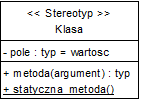
\includegraphics{klasa}
Utworzony został obiekt o identyfikatorze \textbf{Klasa}. Na diagramie będzie to nazwą klasy. Można również nadać inną nazwę korzystając z klucza \textbf{name}(którego nie ma w przykładzie). Klucz \textbf{stereotype} pełni rolę stereotypów w języku UML. Przykładowa klasa posiada metodę(wraz ze statyczną) oraz pole. Na uwagę zasługuje określenie widoczności metod i pól: +, -, ~, \#. Statyczne metody lub pola oznacza się poprzez \_.
Mając już zdefiniowaną klasę \textbf{Klasa} można utworzyć na jej podstawie następny obiekt, kopiując wszystkie ustawione wartości kluczy z \textbf{Klasa}: \textbf{Klasa} NewObject.

\subsubsection{Relacja}

Relację określa się na podstawie prototypu \textbf{relation}.
\begin{lstlisting}
relation
    source-object : Aktor
    source-count : 1
    source-role : "Aktor"

    target-object : uc
    target-count : *
    name : "Uzywa"

actor Aktor
usecase uc
\end{lstlisting}
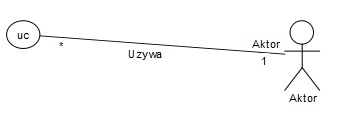
\includegraphics{relacja}
Relację jak wyżej można zdefiniować bez nazwy, jeżeli nie ma potrzeby wykorzystywać do tworzenia nowych obiektów pochodnych od relacji. Klucz \textbf{source-object} wskazuje obiekt na diagramie od którego relacja wychodzi, natomiast \textbf{target-object} wskazuje obiekt docelowy dla końca relacji. Klucze \textbf{source-role} oraz \textbf{target-role} odpowiadają za nadanie obiektowi źródłowemu i docelowemu ról zgodnie z notacją UML. Oczywiście nazwa relacji na diagramie poprzez \textbf{name}. Ponadto relacja może zawierać klucze: \textbf{arror} odpowiadający za określenie rodzaju strzałki relacji oraz \textbf{direction}, który odpowiada za miejsce umieszczenia tej strzałki.

\subsubsection{Asocjacja}

Jako przykład asocjacji można użyć powyższy listing. Oczywiście należałoby zmienić \textbf{relation} na \textbf{association}. Oparta jest również na odpowiednim prototypie. Asocjacja ma już na wstępie zdefiniowane klucze: \textbf{arrow} i \textbf{direction}. Można traktować asocjację jako podstawową formę relacji, tzn. bez kierunków.

\subsubsection{Generalizacja}

Jest relacją o określonym zwrocie i kierunku strzałki.
\begin{lstlisting}
generalization
    source-object : Aktor
    target-object: Klasa

actor Aktor
class Klasa
\end{lstlisting}
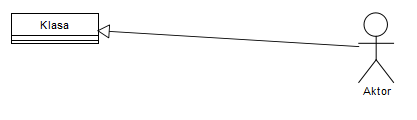
\includegraphics{generalizacja}

\subsubsection{Agregacja}

Różni się od generalizacji typem strzałki oraz jej kierunkiem.
\begin{lstlisting}
aggregation
    source-object : Klasa
    target-object: InnaKlasa

class InnaKlasa
class Klasa
\end{lstlisting}
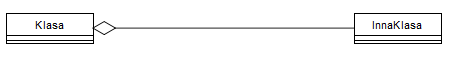
\includegraphics{agregacja}

\subsubsection{Kompozycja}

Kompozycja różni się od generalizacji i agregacji typem strzałki oraz ma kierunek zdefiniowany taki jak agregacja.
\begin{lstlisting}
composition 
    source-object : Aktor
    target-object : Notatka
    
actor Aktor
note Notatka
\end{lstlisting}
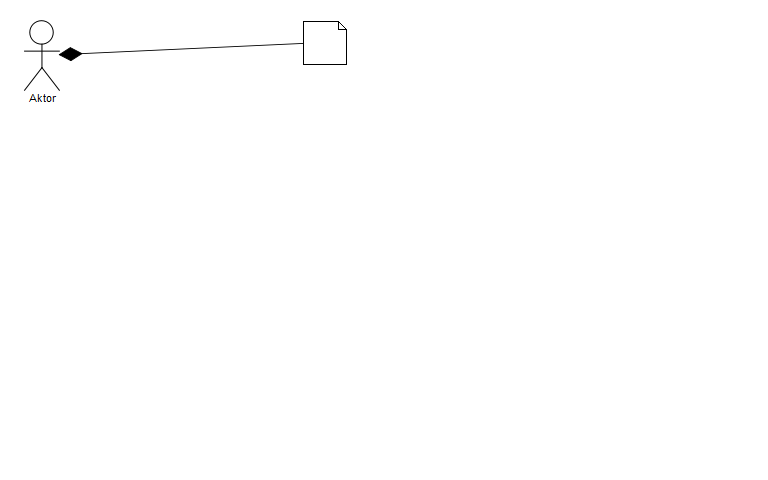
\includegraphics{kompozycja}

\subsubsection{Notatka}

Notatka może posiadać tylko tekst. Nie ma zdefiniowanych innych kluczy oprócz \textbf{text}.
\begin{lstlisting}
note 
    text : "Notatka Notatka Notatka Notatka Notatka Notatka Notatka Notatka"
\end{lstlisting}
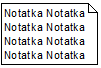
\includegraphics{notatka}

\subsubsection{Aktor i przypadek użycia}

Aktor posiada tylko klucz \textbf{name}. Podobnie przypadek użycia.
\begin{lstlisting}
actor Aktor

usecase uc
    name : "Przypadek uzycia"
\end{lstlisting}
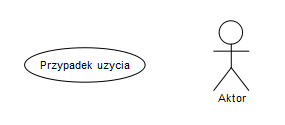
\includegraphics{aktor_uc}